\newcommand{\psd}[1]{{\small\sffamily{\color{blue!60}#1}}}

To showcase the usage of Linear elasticity, we shall discuss here an
example of a 2D bar, which bends under its own load. The bar
\(5\times1\) m\(^2\) in area is made up of material with
\(\rho=8\times 10^3\), \(E=200\times 10^9\), and \(\nu=0.3\).

\begin{figure}[h!]
\centering
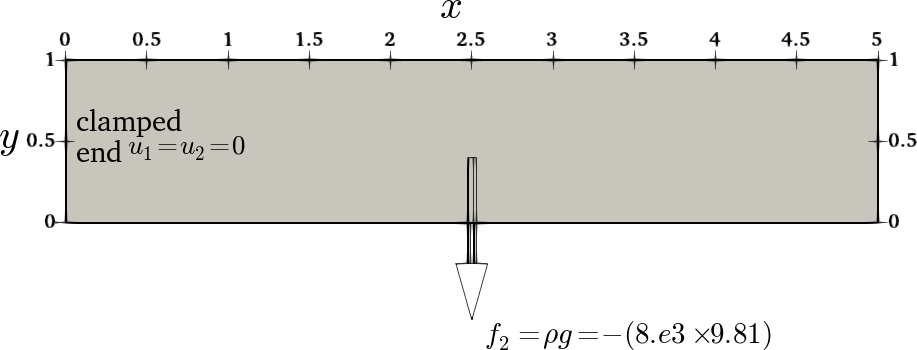
\includegraphics[width=0.5\textwidth]{./Images/le-2d-bar.png}
\caption{The 2D clamped bar problem. \label{2dbar-le-full}}
\end{figure}

\subsection{Step 1: Preprocessing}

First step in a PSD simulation is PSD preprocessing, at this step you
tell PSD what kind of physics, boundary conditions, approximations,
mesh, etc are you expecting to solve.

In the terminal \psd{cd} to the folder
\psd{/home/PSD-tutorials/linear-elasticity}
\footnote{Note that one can perform these simulation in any folder provided that PSD has been properly installed. We use \psd{/home/PSD-tutorials/linear-elasticity} for simplicity, once the user is proficient a simulation can be launch elsewhere.}.
Launch \psd{PSD\_PreProcess} from the terminal, to do so run the
following command.

\begin{lstlisting}[style=BashInputStyle]
PSD_PreProcess -problem linear_elasticity -dimension 2 -bodyforceconditions 1 \
-dirichletconditions 1 -postprocess u
\end{lstlisting}

After the \psd{PSD\_PreProcess} runs successfully you should see many
\psd{.edp} files in your current folder.

\textbf{What do the arguments mean ?}

\begin{itemize}
\item \psd{-problem linear\_elasticity} means that we are solving linear elasticity problem;
\item \psd{-dimension 2} means it is a 2D simulation;
\item \psd{-bodyforceconditions 1} with applied body force acting on the domain;
\item \psd{-dirichletconditions 1} says we have one Dirichlet border;
\item \psd{-postprocess u} means we would like to have ParaView post processing files.
\end{itemize}

At this stage the input properties \(E,\nu\) can be mentioned in
\psd{ControlParameters.edp}, use \psd{E = 200.e9}, and \psd{nu = 0.3;}.
The volumetric body force condition is mentioned in the same file via
variable \psd{Fbc0Fy -78480.0}, i.e (\(\rho*g=8.e3*(-9.81)=-78480.0\)).
One can also provide the mesh to be used in \psd{ControlParameters.edp},
via \psd{ThName = "../Meshes/2D/bar.msh"}
(\textit{note that mesh can also be provided in the next step}) .In
addition variable \psd{Fbc0On 1} has to be provided in order to indicate
the volume (region) for which the body force is acting, here \psd{1} is
the integer volume tag of the mesh. Dirichlet boundary conditions are
also provided in \psd{ControlParameters.edp}. To provide the clamped
boundary condition the variables \psd{Dbc0On 2}, \psd{Dbc0Ux 0.}, and
\psd{Dbc0Uy 0.} are used, which means for Dirichlet border \psd{2}
(\psd{Dbc0On 2}) where \psd{2} is the clamped border label of the mesh
Dirichlet constrain is applied and \psd{Dbc0Ux 0.}, \psd{Dbc0Uy 0} i.e.,
the clamped end condition (\(u_x=u_y=0\)).

\subsection{Step 2: Solving}

As PSD is a parallel solver, let us use 4 cores to solve the 2D bar
case. To do so enter the following command:

\begin{lstlisting}[style=BashInputStyle]
PSD_Solve -np 4 Main.edp -mesh ./../Meshes/2D/bar.msh -v 0
\end{lstlisting}

Here \psd{-np 4} denote the argument used to enter the number of
parallel processes (MPI processes) used while solving.
\psd{-mesh ./../Meshes/2D/bar.msh} is used to provide the mesh file to
the solver. \psd{-v 0} denotes the verbosity level on screen.
\psd{PSD\_Solve} is a wrapper around \psd{FreeFem++} or
\psd{FreeFem++-mpi}. Note that if your problem is large use more cores.
PSD has been tested upto 13,000 parallel processes and problem sizes
with billions of unknowns, surely you will now need that many for the 2D
bar problem.

\subsection{Step 3: Postprocessing}

PSD allows postprocessing of results in ParaView. After the step 2
mentioned above finishes. Launch ParaView and have a look at the
\psd{.pvd} file in the \psd{VTUs...} folder. Using ParaView for
postprocessing the results that are provided in the \psd{VTUs...}
folder, results such as those shown in
figure\textasciitilde{}\ref{bar-le-full} can be extracted.

\begin{figure}[h!]
\centering
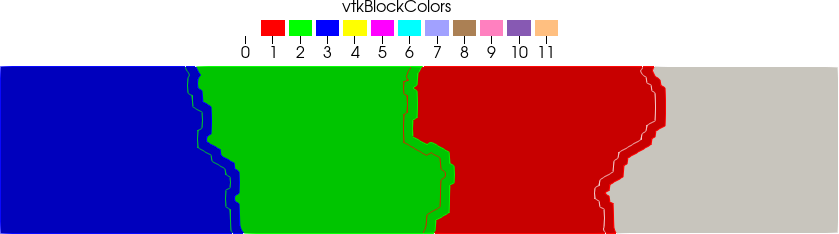
\includegraphics[width=0.4\textwidth]{./Images/le-2d-bar-partioned.png}\\
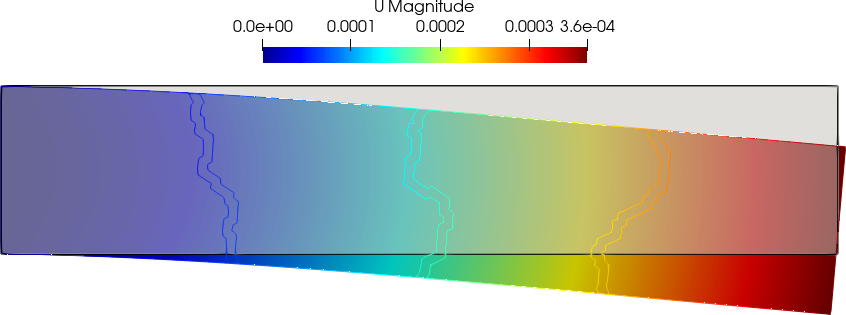
\includegraphics[width=0.4\textwidth]{./Images/le-2d-bar-results.png}
\caption{The 2D clamped bar problem: partitioned mesh and displacement field visualization in ParaView. \label{bar-le-full}}
\end{figure}

You are all done with your 2D linear-elasticty simulation.

\subsection{2D bar is ok, but what about 3D ?}

3D follows the same logic as 2D, in the preprocessing step

\begin{lstlisting}[style=BashInputStyle]
PSD_PreProcess -problem linear_elasticity -dimension 3 -bodyforceconditions 1 \
-dirichletconditions 1 -postprocess u
\end{lstlisting}

note that all what has changed \psd{-dimension 3} instead of
\psd{-dimension 2}

Solving step remains exactly the same with \psd{-mesh} flag now pointing
towards the \psd{3D} mesh.

\begin{lstlisting}[style=BashInputStyle]
PSD_Solve -np 4 Main.edp -mesh ./../Meshes/3D/bar.msh -v 0
\end{lstlisting}

\begin{figure}[h!]
\centering
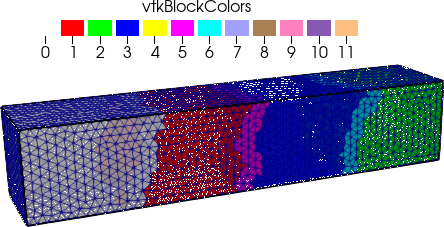
\includegraphics[width=0.4\textwidth]{./Images/le-3d-bar-clamped-ends.png}\\
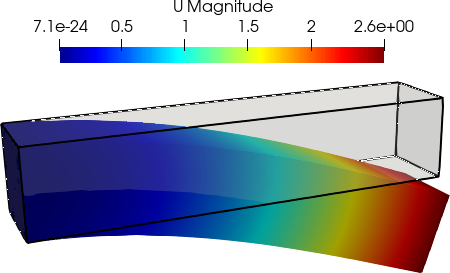
\includegraphics[width=0.4\textwidth]{./Images/le-3d-bar-clamped-pulled-partioned.png}
\caption{The 3D clamped bar problem: partitioned mesh and displacement field visualization in ParaView. \label{3dbar-le-full}}
\end{figure}

Using ParaView for postprocessing the results that are provided in the
\psd{VTUs...} folder, results such as those shown in
figure\textasciitilde{}\ref{3dbar-le-full} can be extracted.
